\section{Данные и их обработка}
Работа производилась со "sky rectified"$\textrm{ }$ изображениями (с уже вычтенным фоном неба), полученными в рамках IAC Stripe 82 Legacy Project.  Используемые фильтры: gri (этап с созданием цветных RGB изображений, фотометрическая декомпозиция), rdeep (этапы с созданием масок, суммарных изображений). 
В процессе выполнения работы были написаны python-скрипты для маскирования, отбора, классификации галактик, скачивания данных, склейки полей.
Для обработки изображений (центрирование на объект, разворот галактики, обрезка изображения, создание rgb изображений, создание суммарных изображений) был использован полуавтоматический пакет для обработки и анализа изображений IMage ANalysis (IMAN)\footnote{\url{https://bitbucket.org/mosenkov/iman_new/src/master/}} и дополнительные python-скрипты. 

С учетом того, что использовались sky rectified изображения, вычет фона неба не производился. Порядок действий по обработке изображений, проводимый в процессе данной работы выглядит следующим образом:
\begin{enumerate}
    \item \textit{Загрузка данных}. Из IAC Stripe 82 Legacy Project были загружены поля в фильтрах r,g,b,rdeep, файлы с psf изображением \footnote{psf (point spread function) -- изображения, описывающие картину, получаемую системой формирования изображения при наблюдении точечного источника или точечного объекта.}, weight-изображения \footnote{weight - изображения, это така называемые карты весов. Имеют тот же размер, что и соответствующее ему изображение с исследуемой галактикой. Только если в обычном fits-изображении с галактикой каждому пикселю соответсвует его значение интенсивности, то в случае weight-файла, каждому пикселю соответсвует его "вес". Этот "вес" вычисляется как $w_i = 1/\sigma_i^2.$
i }
    \item \textit{Первичная обрезка изображения} в фильтрах g,r,i,rdeep с центрирование на объект. Зная координаты центра галактики мы можем вырезать из скачанного поля квадрат, достаточно большой, чтобы не потерять в процессе дальнешей обработки структуры низкой поверхностной яркости и части галактики (квадрат со стороной $\approx$ 10 размеров большой полуоси галактики). Данный этап позволяет быстрее выполнить последующие этапы обработки, например, разворот изображение вокруг центра галактики.
    \item \textit{Разворот галактики}, чтобы та располагалась горизонтально на изображении. На данном этапе используем известные нам значения позиционных углов. В процессе выполнения работы было обнаружено, что примерно для 40 $\%$ выборки изначальные значения PA, определеные при промощи SExtractor, являются неточными. Поэтому для данной категории объектов углы были переопределены методом вписывания эллипса, описывающего внешние изофоты галактики, в программе SAOImage DS9 \cite{2003ASPC..295..489J}. Новые значения позиционных углов были внесены в таблицу и использованы при повторном развороте изображений и анализе параметров объектов выборки.
    \item \textit{Конечная обрезка изображений}. Размер полученного поля составляет 6 размеров больших полуосей галактик. 
    \item \textit{Загрузка соседних полей} в случае, когда галактика находится на границе полей. Склейка осуществлялась при помощи программы SWarp. После осуществлялся повтор предыдущих шагов (обрезка, разворот). Все этапы с центрированием, обрезкой и разворотом производились также с weight-файлами, чтобы в результате каждому пикселю на изображении с галактикой соответствовал его вес в weight-файле.
    \item \textit{Создание масок}. Для данного этапа была создана программа, написанная на языке программирования python. Основной пакет, используемый в скрипте, это пакет \textit{photutils}. Он позволяет выделить на изображении некоторые сегменты, отличающиеся друг от друга по яркости. Каждому сегменту на сегментационной карте соответсвует определенный индекс. В случае, когда сторонний источник находится очень близко к галактике или даже проецируется на нее (то есть перекрывает ее тело), мы можем использовать "деблендинг", то есть разделение сегментов на еще меньшие сегменты, чтобы выделить из них относящиеся к галактике, и не относящиеся к ней. Удаляя из сегментационной карты все сегменты, относящиеся к исследуемому объекту, и оставляя сегменты, покрывающие сторонние источники, мы ликвидируем вклад излучения других объектов из анализа. Пример сегментационной карты, изображения, с наложенной маской приведен на рисунке \ref{fig:mask}.
    \item Создание суммарных\footnote{Суммарное изображение представляет собой сумму изображений в фильтрах r,g,b. Оно является более глубоким и контрасным, позволяющим более чётко видеть структуры низкой поверхностной яркости.} изображений, цветных RGB \footnote{Принцип создания RGB изображения основывается на принципе, в соответствии с которым каждому значению цвета пикселя (например, g-r или r-i) соответствует уникальный цвет на RGB изображении.} изображений.
    \item \textit{Обрезка и разворот}, выполненные для последующей фотометрической декомпозиции. На этом этапе важно, чтобы тело галактики занимало большую часть изображения, что ускоряет сам процесс декомпозиции и минимизирует возможность соседних объектов влиять на результат. Поэтому итоговый размер прямоугольного изображения составляет 3 соответсвующих полуосей галактики для каждой из сторон.
\end{enumerate}

\begin{figure}[ht]

    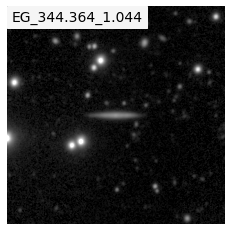
\includegraphics[width=.33\textwidth]{images/data_no_mask.png}\hfill
    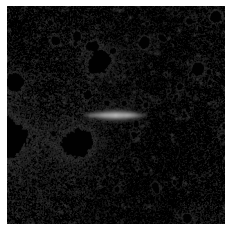
\includegraphics[width=.33\textwidth]{images/data_with_mask.png}\hfill
    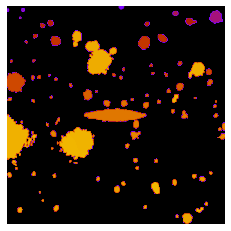
\includegraphics[width=.33\textwidth]{images/segm.png}\hfill

    \caption{Левая панель -- пример изображения галактики из выборки, центральная панель -- изображение той же галактики с наложенной маской, правая панель -- сегментационная карта для этой же галактики. }\label{fig:mask}
\end{figure}
